\documentclass{beamer}
\usepackage{amsmath,amsbsy,amsopn,amstext,amsfonts,amssymb}
\usepackage{isomath}
\usepackage{ulem}
%\linespread{1.6}  % double spaces lines
\usepackage{graphicx}
\usepackage{subfigure}
\usepackage{color}
\usepackage{optidef}  % define optimization problems
\usepackage{multicol}  % multiple columns
\usepackage{listings} % for python code
\usepackage{mathrsfs}

\usepackage{polynom}
\newcommand{\adj}{\mathrm{adj}}
\newcommand{\constrainedmin}[3]{
		\begin{mini*}|s|
		{#2}{#1}{}{}
		\addConstraint{#3}
		\end{mini*}
}

\newcommand{\rwbcomment}[1]{{\color{blue}RWB:#1}}
\newcommand{\defeq}{\stackrel{\triangle}{=}}
\newcommand{\abs}[1]{\left|#1\right|}
\newcommand{\norm}[1]{\left\|#1\right\|}
\newcommand{\iprod}[1]{\left<#1\right>}
\newcommand{\ellbf}{\boldsymbol{\ell}}
\newcommand{\nubf}{\boldsymbol{\nu}}
\newcommand{\mubf}{\boldsymbol{\mu}}
\newcommand{\abf}{\mathbf{a}}
\newcommand{\bbf}{\mathbf{b}}
\newcommand{\cbf}{\mathbf{c}}
\newcommand{\dbf}{\mathbf{d}}
\newcommand{\ebf}{\mathbf{e}}
\newcommand{\fbf}{\mathbf{f}}
\newcommand{\gbf}{\mathbf{g}}
\newcommand{\hbf}{\mathbf{h}}
\newcommand{\ibf}{\mathbf{i}}
\newcommand{\jbf}{\mathbf{j}}
\newcommand{\kbf}{\mathbf{k}}
\newcommand{\lbf}{\mathbf{l}}
\newcommand{\mbf}{\mathbf{m}}
\newcommand{\nbf}{\mathbf{n}}
\newcommand{\obf}{\mathbf{o}}
\newcommand{\pbf}{\mathbf{p}}
\newcommand{\qbf}{\mathbf{q}}
\newcommand{\rbf}{\mathbf{r}}
\newcommand{\sbf}{\mathbf{s}}
\newcommand{\tbf}{\mathbf{t}}
\newcommand{\ubf}{\mathbf{u}}
\newcommand{\vbf}{\mathbf{v}}
\newcommand{\wbf}{\mathbf{w}}
\newcommand{\xbf}{\mathbf{x}}
\newcommand{\ybf}{\mathbf{y}}
\newcommand{\zbf}{\mathbf{z}}
\newcommand{\Jbf}{\mathbf{J}}
\newcommand{\Acal}{\mathcal{A}}
\newcommand{\Bcal}{\mathcal{B}}
\newcommand{\Lcal}{\mathcal{L}}
\newcommand{\Ncal}{\mathcal{N}}
\newcommand{\Rcal}{\mathcal{R}}
\definecolor{darkolivegreen}{rgb}{0.33, 0.42, 0.18}

\makeatletter
\newenvironment<>{proofstart}[1][\proofname]{%
    \par
    \def\insertproofname{#1\@addpunct{.}}%
    \usebeamertemplate{proof begin}#2}
  {\usebeamertemplate{proof end}}
\newenvironment<>{proofcont}{%
  \setbeamertemplate{proof begin}{\begin{block}{}}
    \par
    \usebeamertemplate{proof begin}}
  {\usebeamertemplate{proof end}}
\newenvironment<>{proofend}{%
    \par
    \pushQED{\qed}
    \setbeamertemplate{proof begin}{\begin{block}{}}
    \usebeamertemplate{proof begin}}
  {\popQED\usebeamertemplate{proof end}}
\makeatother

\title{ECEn 671: Mathematics of Signals and Systems}
\author{Randal W. Beard}
\institute{Brigham Young University}
\date{\today}

\begin{document}

%-------------------------------
\begin{frame}
	\titlepage
\end{frame}

%%%%%%%%%%%%%%%%%%%%%%%%%%%%%%%%%%%%%%%%%%%%%%%%%%%%%%%%%%%%%%%%%%%%%%%
\section{Normed Spaces}
\frame{\sectionpage}

%----------------------------------
\begin{frame}\frametitle{Norms and Normed Spaces}
\begin{definition}[Norm] Let $S$ be a vector space, $\norm{ x }$ is a norm if:
\begin{flalign*}
(N1) \qquad & \norm{ x } \geq 0 \quad \forall x \in S\\
(N2) \qquad & \norm{ x } = 0 \quad \Leftrightarrow x = 0\\
(N3) \qquad & \norm{ \alpha x } = \alpha\norm{ x }\\
(N4) \qquad & \norm{ x + y } \leq \norm{ x } + \norm{ y }\quad \text{(triangle inequality)}\\
\end{flalign*}
\end{definition}
\end{frame}

%----------------------------------
\begin{frame}\frametitle{Differences between norms and metrics:}
\begin{itemize}
\item Norms only have one argument (the length of a vector), where metrics are distances between elements of a set.
\item Norms are only defined for vector spaces!\\
(i.e. there is no norm for rotation matrices, but there are metrics!)
\item Norms scale with the vector (N3)\\
(there are metrics that don't scale), e.g. $d(x,y) = \begin{cases} 1 \quad x &\neq y\\0 \quad x &= y\end{cases}$
\item Every norm is also a metric\\
\[ \norm{ x - y } = d(x,y) \]
\[ \norm{ x } = d(x,0) \]
\end{itemize}
\end{frame}

%----------------------------------
\begin{frame}\frametitle{Definition: Normed Space} 

A \underline{normed} space is a pair $(\mathbb{X},\norm{ \cdot} )$ where $\mathbb{X}$ is a vector space and $\norm{ \cdot} $ is a norm.

\begin{example}[Normed Spaces]
$\mathbb{R}^n$ is a vector space.  All of the following norms are valid:
\begin{itemize}
  \item one-norm \quad $\norm{ x}_1 = \displaystyle \sum_{i=1}^{n}|x_i|$ \quad (power vectors)
  \item two-norm \quad $\norm{ x}_2 = \displaystyle \left( \sum_{i=1}^{n}|x_i|^2 \right)^{\frac{1}{2}}$ \quad (energy vectors)
  \item infinity-norm \quad $\norm{ x}_{\infty} = \underset{i=1,\cdots,n}{\max}|x_i|$ \quad (bounded vectors)
  \item p-norm \quad $\norm{ x}_p = \left( \displaystyle \sum_{i=1}^{n}|x_i|^p \right)^{\frac{1}{p}}$
\end{itemize}
\end{example}
\end{frame}

%----------------------------------
\begin{frame}\frametitle{Unit Circle in $\mathbb{R}^2$}

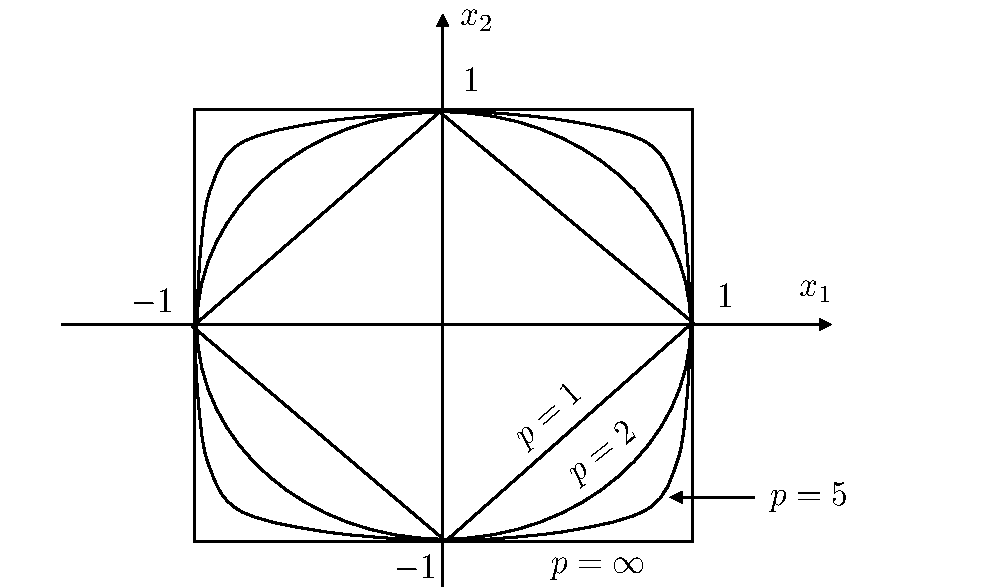
\includegraphics[width=0.9\textwidth]{figures/chap2_unit_circle}\\
	
\end{frame}
 

%----------------------------------
\begin{frame}\frametitle{Normed Space Example: Sequence Spaces}
Let $\boldsymbol{\ell}$ be the set of sequences: $x = (x_1, x_2, x_3, \cdots)$.  
The following normed vector spaces can be defined:
\begin{itemize}
\item $\boldsymbol{\ell}_1$: (power sequences)  If $\norm{ x}_{\ell_1} = \sum_{i=1}^{\infty}|x_i|$ then 
$\boldsymbol{\ell}_1 \defeq \{x \in \boldsymbol{\ell} : \norm{x}_{\ell_1} < \infty \}$
\item $\boldsymbol{\ell}_2$: (energy sequences)  If $\norm{ x}_{\ell_2} = \left(\sum_{i=1}^{\infty}|x_i|^2\right)^{1/2}$ then $\boldsymbol{\ell}_2 \defeq \{x \in \boldsymbol{\ell} : \norm{x}_{\ell_2} < \infty \}$
\item $\boldsymbol{\ell}_\infty$: (bounded sequences)  If $\norm{ x}_{\ell_\infty} = \sup_{j\in\mathbb{N}}|x_j|$ then $\boldsymbol{\ell}_\infty \defeq \{x \in \boldsymbol{\ell} : \norm{x}_{\ell_\infty} < \infty \}$
\item $\boldsymbol{\ell}_p$:  If $\norm{ x}_{\ell_p} = \left(\sum_{i=1}^{\infty}|x_i|^p\right)^{1/p}$ then $\boldsymbol{\ell}_p \defeq \{x \in \boldsymbol{\ell} : \norm{x}_{\ell_p} < \infty \}$ for $1\leq p \leq\infty$
\end{itemize}
\end{frame}

%----------------------------------
\begin{frame}\frametitle{Normed Space Examples}

\begin{example}
Consider the sequence $x = (1,1,1,\ldots)$:
\begin{itemize}
\item $x \in \boldsymbol{\ell}_{\infty}$, but
\item $x \notin \boldsymbol{\ell}_p \text{ for } 1 \leq p < \infty$.
\end{itemize}
\end{example}

\begin{example}
Consider the sequence $x = (1, \frac{1}{2}, \frac{1}{3}, \frac{1}{4}, \ldots)$
\begin{itemize}
\item 	$x \notin \boldsymbol{\ell}_1$ (prove this), but 
\item $x \in \boldsymbol{\ell}_p \quad p > 1$ (prove this)
\end{itemize}
\end{example}
\end{frame}

%----------------------------------
\begin{frame}\frametitle{Normed Space Example: Function Spaces}
Let $L^n(\Omega)$ be the set of functions on $\Omega$. $x\in L^n(\Omega)$ is an equivalent classes of functions, i.e. equal except on a set of measure zero.  (picture)  The following norms are valid:
\begin{itemize}
\item 	$L_1^n(\Omega)$ (power signals).  If $\norm{x}_{L_1^n(\Omega)} = \int_{\Omega}\norm{ x(t)}  dt$, then $L_1^n(\Omega) = \{ x\in L^n(\Omega)| \norm{x}_{L_1^n(\Omega)} < \infty \}$.
\item $L_2^n(\Omega)$ (energy signals).  If $\norm{x}_{L_2^n(\Omega)} = \left(\int_{\Omega}\norm{ x(t)}^2  dt\right)^{1/2}$, then $L_2^n(\Omega) = \{ x\in L^n(\Omega)| \norm{x}_{L_2^n(\Omega)} < \infty \}$.
\item $L_p^n(\Omega)$.  If $\norm{x}_{L_p^n(\Omega)} = \left(\int_{\Omega}\norm{ x(t)}^p  dt\right)^{1/p}$, then $L_p^n(\Omega) = \{ x\in L^n(\Omega)| \norm{x}_{L_p^n(\Omega)} < \infty \}$, $1\leq p \leq \infty$.
\item 	$L_\infty^n(\Omega)$ (bounded signals).  If $\norm{x}_{L_\infty^n(\Omega)} = \sup_{t\in\Omega}\norm{ x(t)}$, then $L_\infty^n(\Omega) = \{ x\in L^n(\Omega)| \norm{x}_{L_\infty^n(\Omega)} < \infty \}$.
\end{itemize}
\end{frame}


\end{document}